\documentclass[12pt, a4paper]{article}
\usepackage[utf8x]{inputenc}
\usepackage{ragged2e}
\usepackage{amsmath}
\usepackage{pdflscape}
\usepackage{graphicx}
\usepackage{hyperref}
\usepackage{subcaption}
\graphicspath{ {./images/} }
\usepackage{geometry}
\renewcommand{\refname}{Referanslar}
\renewcommand{\contentsname}{İçindekiler Tablosu}
\usepackage[ddmmyyyy]{datetime}
\renewcommand{\dateseparator}{.}
\renewcommand{\figurename}{Şekil}
\renewcommand{\abstractname}{Özet}
\renewcommand{\tablename}{Tablo}
\renewcommand{\thesection}{\arabic{section}}
\renewcommand{\thesubsection}{\arabic{subsection}}
\renewcommand{\thesubsubsection}{\arabic{subsubsection}}
\geometry{
	top=2.5cm,
	left=2.5cm,
	right=2.5cm,
	bottom=2.5cm
}
\begin{document}
	\begin{titlepage}
		\centering
		{\LARGE TRAFİKTE YORGUNLUK TESPİT SİSTEMİ DOKÜMANI \par}
		\vspace{1cm}
		{\Large Sema YEŞİLKAYA \par}
		\vspace{1.5cm}
		\begin{abstract}
			
			Sürücünün yorgunluğunu algılama projesi, trafikteki kaza oranlarının belirli bir yoğunluğunun yorgun sürücülerden oluşması dolayısıyla önem kazanmaktadır.Bu projenin amacı yorgun sürücüleri algılayıp onları dinlenmeye yönlendirme veya araç kullanmayı bıraktırma gibi koşulların sıklığına bağlı olarak sonuçların da değişmesidir.\newline Bu çalışamada Opencv kullanılmıştır. Opencv aracılığıyla yüzdeki bölgelerin seçilmesi sağlanıp frameler olarak işleme alınması sağlanmıştır.Çalışma yüksek doğrulukla çalışmaktadır. Gözlük,esnerken ağız kapatma, kişilerin göz farklılığı gibi durumlar göz önüne alınarak hazırlandığı için doğruluğa yakın olarak tasarlanmıştır.Sonuçlar da gösteriyor ki yorgun sürücülerde belirtilen koşullar ele alınırsa daha sağlıklı ve bilinçli bir trafikte bulunulacaktır. \newline
			Anahtar Kelimeler: Sürücü yorgunluğu, Opencv, Cascade.
		\end{abstract}
		\vfill
	\end{titlepage}
	
	\tableofcontents
	\newpage
	
	\section{Giriş}
	\pagenumbering{arabic}
	Günümüzde trafik güvenliği, toplumun en önemli meselelerinden biri haline gelmiştir. Trafik kazalarının önemli bir kısmının yorgun sürücülerden kaynaklandığı bilinmektedir. Bu çalışma, yorgun sürücüleri etkin bir şekilde tespit ederek trafikteki kaza oranlarını azaltmayı amaçlamaktadır. Yorgunluk, sürücünün tepki süresini yavaşlatır ve karar verme yeteneğini olumsuz etkiler, bu da potansiyel olarak tehlikeli durumlara yol açabilir. Bu nedenle, yorgun sürücülerin erken tespiti, trafik güvenliğini artırmada kritik bir rol oynamaktadır.
	
	Bu çalışmanın motivasyonu, trafik kazalarını önleme ve yollarımızı daha güvenli hale getirme arzusundan kaynaklanmaktadır. Yorgunluk algılama sistemlerinin geliştirilmesi, sürücülerin dinlenmeye yönlendirilmesi veya araç kullanmayı bırakmaları konusunda \newline uyarılmasını sağlayarak, trafikteki güvenliği artırabilir.
	
	OpenCV kütüphanesi kullanılarak geliştirilen bu sistem, yüz tanıma ve görüntü işleme tekniklerini kullanarak sürücünün yorgunluk seviyesini belirlemektedir. Gözlük takma, esneme sırasında ağız kapatma ve kişisel göz farklılıkları gibi faktörler dikkate alınarak tasarlanmıştır. Bu sayede, sistem yüksek doğrulukla çalışmakta ve çeşitli koşullarda güvenilir sonuçlar üretmektedir.
	
	Literatürdeki mevcut çalışmalar, yorgunluk algılama konusunda çeşitli yöntemler önermiş olsa da, bu çalışma, yüz tanıma teknolojisindeki son gelişmeleri ve görüntü işleme algoritmalarını birleştirerek, daha etkin ve doğru bir çözüm sunmayı hedeflemektedir. Bu çalışma, yorgun sürücüleri algılama konusunda literatüre önemli katkılarda bulunmayı ve trafik güvenliğini artırmayı amaçlamaktadır.
	
	\section{Yöntem}

	\begin{itemize}
		
	\item Yüz tanıma: Cascade \newline
	Cascade yüz tanıma yöntemi, nesne tanıma alanında oldukça yaygın olarak kullanılan bir yöntemdir.
	Temel olarak, bir yüzün farklı özelliklerini (gözler, burun, ağız vb.) tanımak için bir dizi önceden eğitilmiş sınıflandırıcıdan oluşur.
	Bu sınıflandırıcılar, yüzün farklı bölgelerini tarar ve yüzün varlığını veya yokluğunu belirlemeye çalışır.
	Cascade yöntemi, hızlı çalışma süresi ve yüksek doğruluk seviyeleri nedeniyle tercih edilir.
	\item Tanınan yüzden gözleri ayırt etme : Cascade  \newline
	Cascade yöntemi, yüz tanıma işlemi sırasında gözleri ayırt etmek için de kullanılır.
	Gözleri ayırt etmek için yine önceden eğitilmiş sınıflandırıcılar kullanılır.
	Bu sınıflandırıcılar, gözlerin varlığını veya yokluğunu tespit eder ve yüz tanıma sistemine daha fazla bilgi sağlar.
	\item Göz durumlarının sınıflandırılması : SVM+ HOG  \newline
	Destek vektör makinesi (Support Vector Machine,SVM), nesne tanıma ve sınıflandırma için kullanılır. Nesnelerin farklı bölümlerini (örneğin gözler, burun, ağız) tanımak için deformable part model kullanır.
	HOG, nesnelerin kenarlarını ve şekillerini tanımak için kullanılır. Göz durumlarını sınıflandırmak için kullanılabilir.
	\item Yorgunluk Tespiti : Perclos
	Sürücülerin yorgunluk seviyelerini tespit etmek için kullanılır.
	Sürücünün göz kapanma oranını (gözlerin ne kadar süreyle kapalı olduğunu) hesaplar.
	Yüksek Perclos değerleri, sürücünün yorgun olduğunu ve dikkatinin dağıldığını gösterebilir. Yöntemler genel olarak \cite{ieeedata} baz alınarak belirlenmiştir.
	\begin{equation}\label{Perclos}
		P = \frac{\text{kapalı göz içeren kare sayısı}}{\text{toplam kare sayısı}} \times 100
	\end{equation}
	Yukarıdaki (\ref{Perclos}) numaralı eşitlik Perclos değerinin nasıl hesaplanacağını gösterir.
	\begin{figure}[!h]
		\centering
		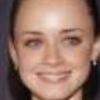
\includegraphics[width=14cm, height=7cm, keepaspectratio]{Alexis_Bledel_0001.jpg}
		\caption{Veri setinden açık gözlü yüz örneği \cite{mrl}.}\end{figure}
		\begin{figure}[!h]
		\centering
		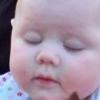
\includegraphics[width=17cm, height=7cm, keepaspectratio]{closed_eye_0047.jpg_face_2.jpg}
		\caption{Veri setinden kapalı gözlü yüz örneği \cite{mrl}.} 
		\end{figure}\par
	\end{itemize}
	\section{Bulgu ve Tartışma}
	Projede kullanabilmek için dlib kütüphanesi import edilmiştir . Dlib yüz tanımlama gibi pek çok yerde kullanılan geniş kapsamlı ve açık kaynaklı bir kütüphanedir.\par Bilgisayarımda başka bir python sürümü(3.9) bulunması gerekmektedir ve bunu standart olarak kullanabilmek için path olarak eklenmiştir. Fakat yine de olumlu bir sonuç elde edilmemiştir. \begin{figure}[!h]
		\centering
		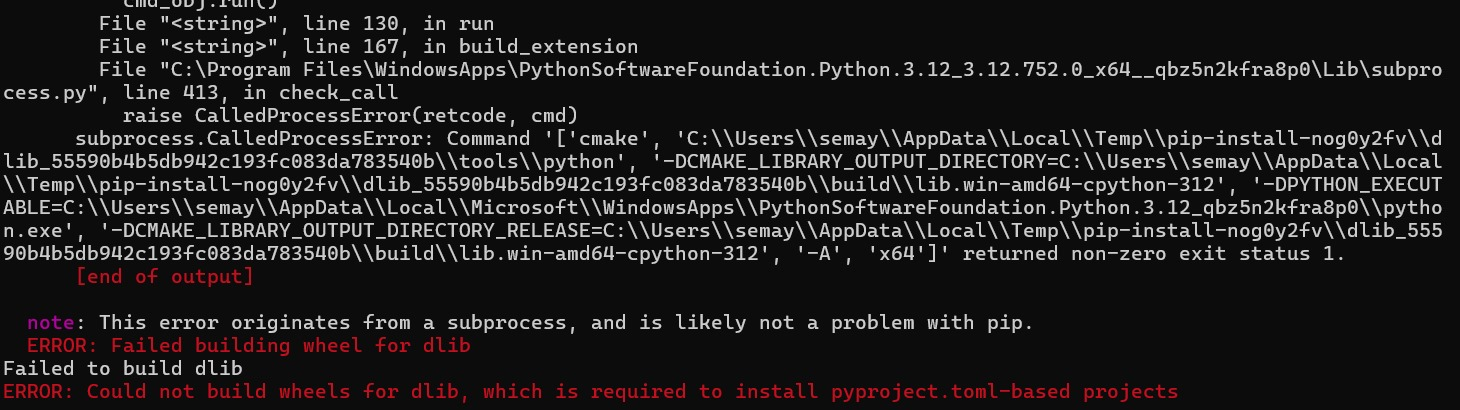
\includegraphics[width=17cm, height=7cm, keepaspectratio]{error.jpg}
		\caption{Alınan hata.} 
	\end{figure}\par \begin{figure}[!h]
		\centering
		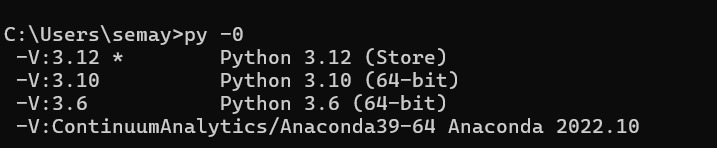
\includegraphics[width=17cm, height=7cm, keepaspectratio]{psurumu.jpg}
		\caption{Python sürümleri.} 
	\end{figure}\par
	Bilgisayarda yaşanan sürüm uyuşmazlığı çözülemediği için dlib olmadan bu projenin nasıl yapıldığı araştırıldı. Sadece Opencv import ederek yani import cv2 komutuyla yapılan bir kod örneği incelendi ve Haarcascade ile de çalışıldığını görüldü.\newline
	Haarcascade için hazır kodların yanında kendimiz de oluşturabiliriz. Pozitif ve negatif resimlere ihtiyacımız olur. Bu resimleri etiketleme işlemi gibi işlemden geçirdikten sonra bir tarafa nesnenin varlığını diğer tarafa olmadığını tanıtarak bu belgeler .bat formunda kaydedilir. Sistem tarafından çalıştırılıp tanınması için de .xml uzantısı olarak değiştirilir. Bu değişimi gerekli araçlarla yapabilirsiniz. \cite{dasar_haartrain} burada anlatılan sistemi yararlı bulunmuştur ve ilerleyen süreçte bu veri setini kullanılacaktır.\clearpage
	\begin{figure}
		\centering
		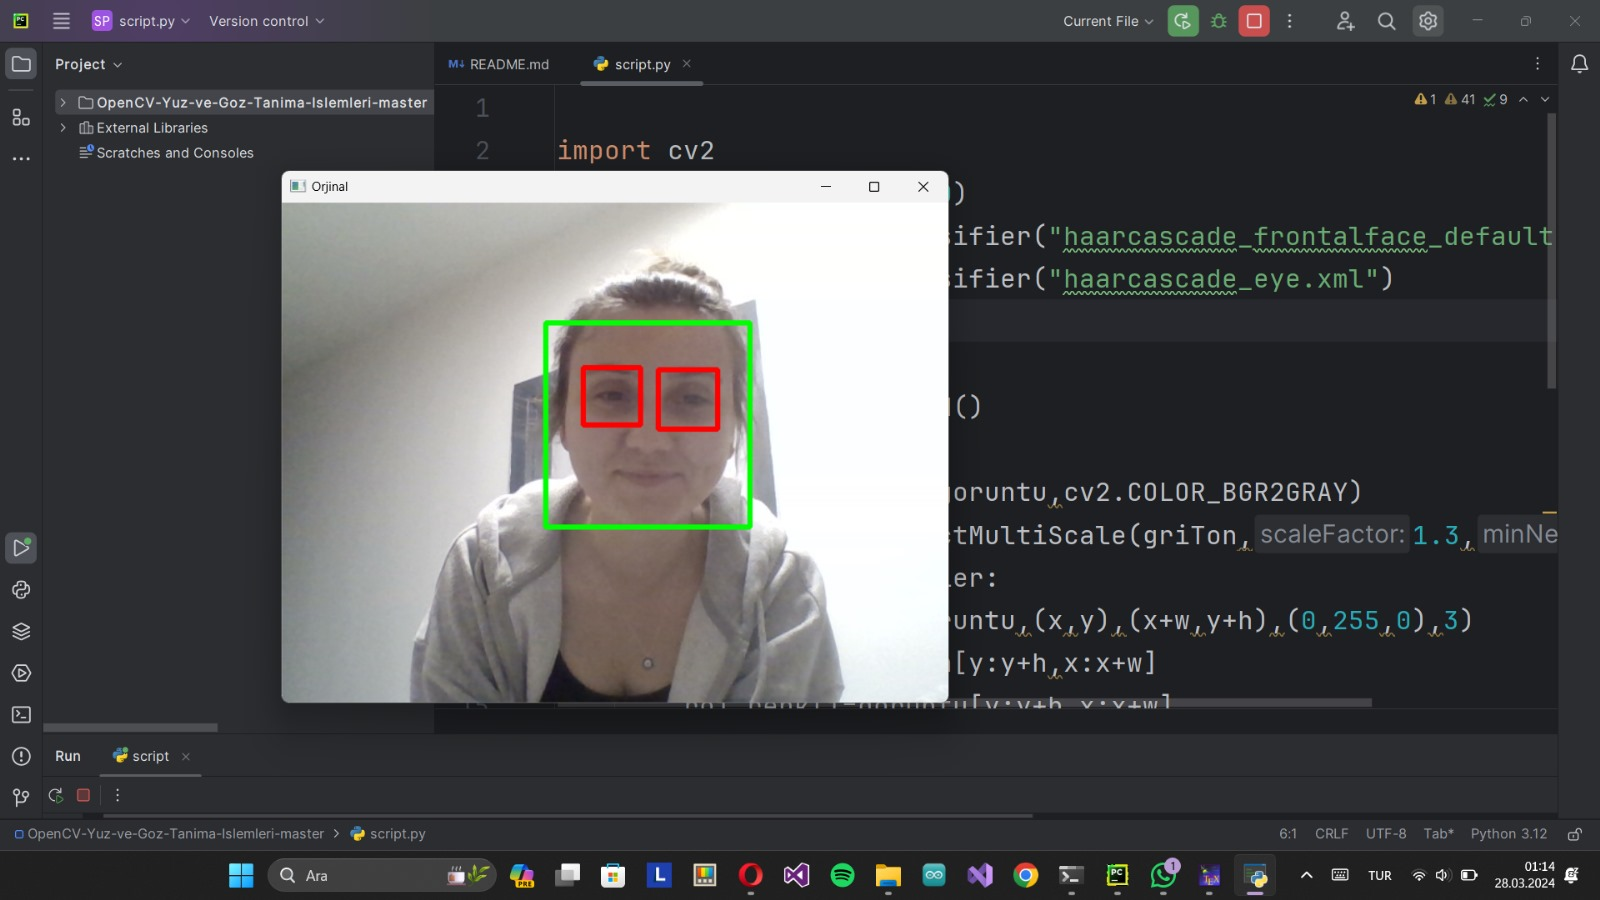
\includegraphics[width=17cm, height=7cm, keepaspectratio]{yuzgoztanima.jpg}
		\caption{Yüz ve göz tespiti.} 
	\end{figure}
	\par
	Bu sisteme göz kapalılığı da eklenecektir.\\ 
   \subsection{Göz Kapalılığı Tespiti}
   Göz kapalılığını hesaplarken gözün etrafında bulunan 6 noktadan faydalanılır. Bu noktalar arası uzaklığını azalması ve belirli eşik değerin altında belirli bir süre kalması durumunda yorgunluk tespit edilmiş demektir. Bu duruma göre numpy ekledim ve hesaplama yaparak göz açıklık kapalılık kodunu yazmaya çalıştım. Kodun çalışması için dlib gerekli.\par
	Dlib kütüphanesini yüklemekle ilgili sorun vardı ve bu sorun çözüldü. Sorunu çözerken işlemlere baştan başlandı.Öncelikle VsCode derleme araçlarını indirildi. Cmake kuruldu. Daha sonra pip install dlib komutuyla bu kütüphaneyi indirildi \cite{onursahin}.İndirip örnek projelerde kullanmaya devam edebilebilirdi fakat dlib olmadan kullanılan projede denendi. Gözün open- close durumlarında hata alındı.\par 
	 Dlib kütüphanesinde landmark denen bir özellik vardır.Dlib kütüphanesindeki “landmark” terimi, yüzdeki belirli noktaları veya bölgeleri tanımlamak için kullanılır.Dlib’in en yaygın kullanılan yüz landmark dedektörü, 68 noktalı bir yapıya sahiptir ve yüzün ana hatlarını hızlı ve güvenilir bir şekilde tespit edebilir. \par Göz mesafesini hesaplamak için kullandığım standart olarak kullanılan eşik değer sabittir.İlerleyen süreçte bu eşik değer değiştirelecektir. Kullanıcıdan ilk önce gözünün açık ve kapalı hallerini isteyerek ona göre hesaplamaya geçilecektir. \newpage
	\begin{figure}
		\centering
		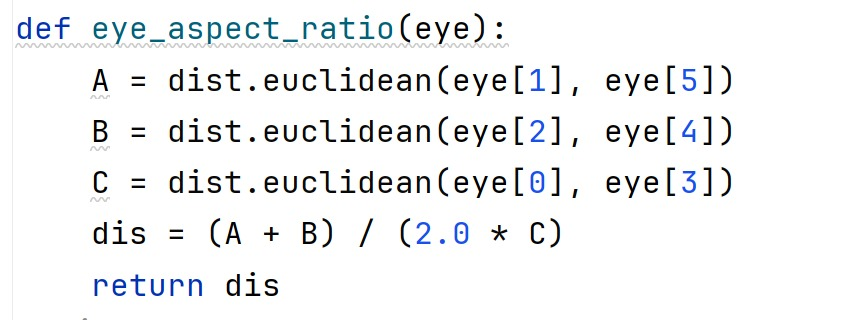
\includegraphics[width=10cm, height=7cm, keepaspectratio]{kod.jpg}
		\caption{Göz mesafesi hesaplama.} 
	\end{figure} \par \begin{figure}[!h]
		\centering
		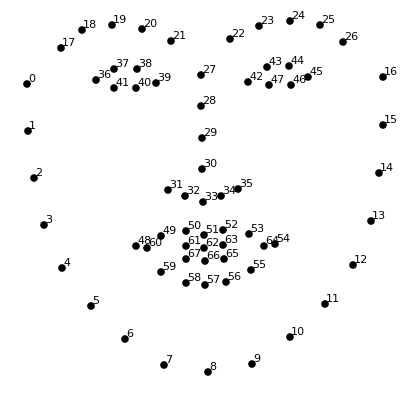
\includegraphics[width=17cm, height=7cm, keepaspectratio]{landmarks.jpg}
		\caption{Göz tespiti için Dlib kütüphanesinin kullandığı landmark değerleri\cite{amos2018}.} 
		\par
	\end{figure} \par
	Projede kullanılan yöntem geleneksel yöntemdir. Bu süreçte amaç, bu yöntem(Haarcascade) ile yeni teknolojilerden birini karşılaştırıp hangisinin daha sağlıklı sonuç verdiğini görmek.
	Yeni yöntem olarak CNN kullanılan bir örnek proje \cite{superthinking} bulundu.
	CNN, yani Evrişimli Sinir Ağları (Convolutional Neural Networks), görüntü işlemede kullanılan bir derin öğrenme algoritmasıdır. Görselleri girdi olarak alır ve farklı operasyonlarla bu görsellerdeki özellikleri (features) yakalar ve sınıflandırır \cite{cnnnedir}. CNN, özellikle görüntü tanıma, nesne tespiti ve benzeri görsel tabanlı görevlerde etkili bir şekilde kullanılır.
	CNN’nin temel bileşenleri şunlardır:
	
	Evrişim Katmanı (Convolutional Layer): Görüntü üzerinde gezinen ve özellikleri yakalayan filtreler içerir.\\
	Aktivasyon Fonksiyonu (ReLU gibi): Modelin doğrusal olmayan özellikleri öğrenmesini sağlar.\\
	Havuzlama Katmanı (Pooling Layer): Görüntü boyutunu küçültür ve özellikleri yoğunlaştırır.\\
	Tam Bağlantılı Katman (Fully Connected Layer): Öğrenilen özellikleri kullanarak sınıflandırma yapar \cite{cnnnedirtek}.\par
	Bu katmanlar, bir görüntünün temel özelliklerinden daha karmaşık özelliklere kadar çeşitli soyutlama seviyelerinde özellikleri öğrenmek için bir arada çalışır. CNN modelleri, bu özellikleri öğrenmek ve güncellemek için eğitim sürecinde sürekli olarak kendilerini iyileştirir.\newpage
	\begin{figure}
		\centering
		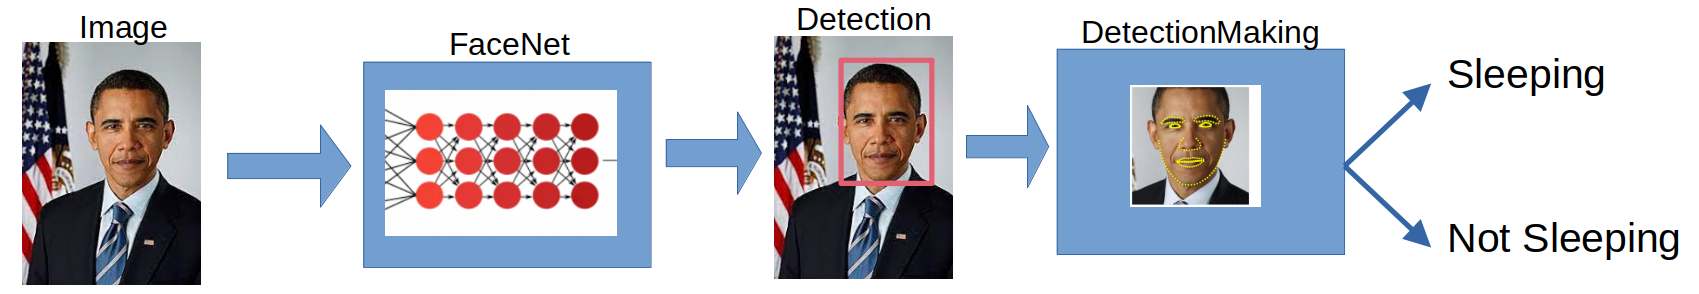
\includegraphics[width=10cm, height=7cm, keepaspectratio]{process.png}
		\caption{CNN ile sürücü yorgunluğu tespiti \cite{eadali}.}
	\end{figure} 
	\begin{table}[h!]
		\begin{center}
			\caption{Haarcascade ve CNN Karşılaştırması.}
			\label{tab:table1}
			\begin{tabular}{l|c|c|}
				\textbf{Özellik} & \textbf{Haarcascade} & \textbf{CNN}\\
				\hline
				Hızlı tespit süresi & Evet & Hayır\\
				Düşük kaynak gereksinimi & Evet & Hayır\\
				Yüksek doğruluk & Hayır & Evet\\
				Özellik mühendisliği gerekmez & Hayır & Evet\\
				Yüksek hesaplama gücü gereksinimi & Hayır & Evet\\
				Uzun eğitim süresi & Hayır & Evet\\
			\end{tabular}
		\end{center}
	\end{table}
	Yukarıda gördüğünüz üzere CNN daha iyi bir sonuç çıkarıyor. Eğer doğruluk önemsenmeseydi Haarcascade kullanılabilirdi.CNN ile yapılmış projede Tensorflow ve Theano yüklemesinde sorun yaşanıldığı için çalıştırılamadı. Cascade için de başın pozisyonunu algılayıp üç boyutlu sisteme dönüştürerek vücut postürünü algılayan fonksiyon eklendi.\par 
	Yeni CNN kodunda Tenforflow sürüm hatası alındı. Thaeno kütüphanesini Numpy ile benzer olması dolayısıyla kaldırıldı.Kod sahibi de Numpy kullanmıştı zaten.Ayrıca göz aralıklarını hesaplayarak gözün kapalı açık durumunu tespit ettiğimiz landmark olarak adlandırdığımız noktalar mantığında ve yine aynı yöntemle, ağız açıklığını tespit eden fonksiyonu da ekleyerek çoklu faktör kontrolü sağlandı. Bu değerlerden 3 veya daha fazlası gerçekleşiyorsa kişi yorgun olarak tanımlanıp konumuna göre en yakın otele yönlendirme yapılıyor.\newpage
	\begin{figure}
		\centering
		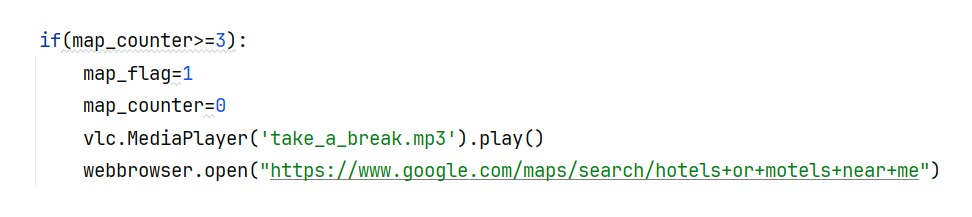
\includegraphics[width=10cm, height=7cm, keepaspectratio]{otel.jpg}
		\caption{Yorgunluk eşiğine göre otele yönlendirme\cite{superthinking}.}
	\end{figure} 
	\begin{figure}
		\centering
		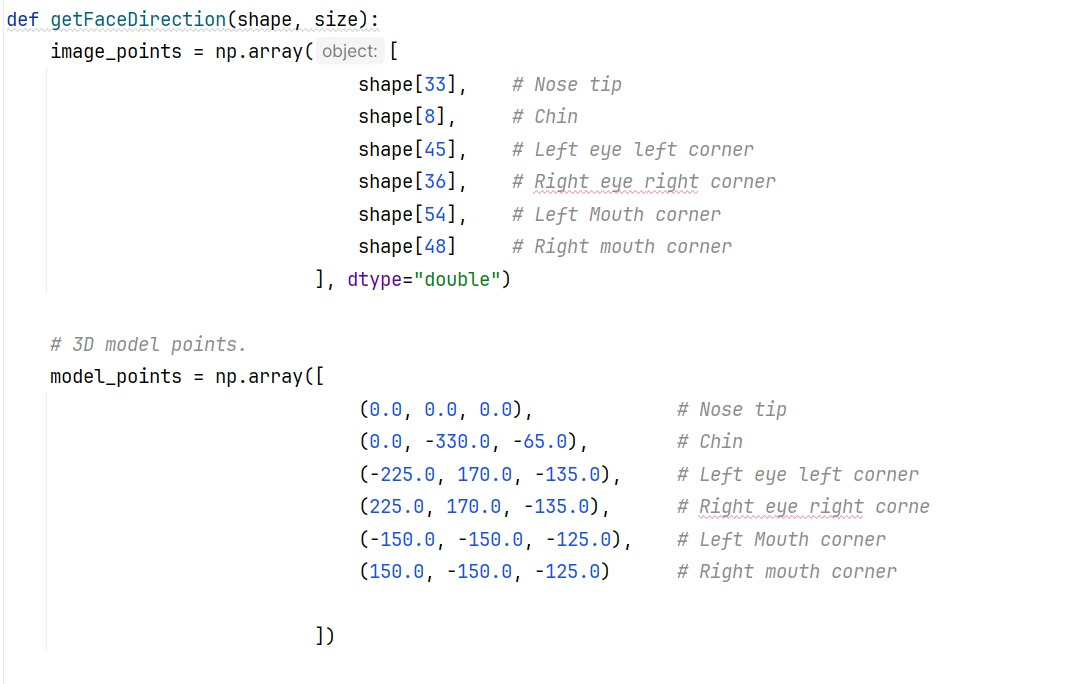
\includegraphics[width=10cm, height=7cm, keepaspectratio]{bastanimlama.jpg}
		\caption{Baş pozisyonu tahmini için tanımlamalar\cite{superthinking}.}
	\end{figure}
	\subsection{ Eşik Değerin Kişileştirilmesi} 
	
	Her insanın göz boyutu farklıdır. Bu durum göz tespit algoritmalarında sorun çıkarmaktadır. Örneğin gözün açıklık kapalılık durumuna göre yorgunluk seviyesi algılanması olgusunda verilen eşik değere göre normalde gözü açık bir bireyin gözü kapalı algılanması olası bir durumdur.\par Belirli bir eşik değere göre sürücünün göz durumunu tespit etmek sağlıklı bir yöntem değildir. Bu sebeple belirli bir eşik değer yerine sürücünün gözünün açık ve kapalı fotoğrafını alıp oranlayıp yeni eşik değer oluşturulmasıyla hesaplanan bir durum daha net sonuçlar elde edilmesine sebep olacaktır.\par Kapalı gözün tespit edilmesiyle kapalı olduğu süre de tespit edilebilir. Böylece sürücüye örneğin 3. saniyede odaklanın gibi bir uyarı verilir. Uyarı verilirken pygame kütüphanesini kullanıldı. Playsound kütüphanesi yaygın kullanılıyordu fakat entegre etmekte hata alındı ve hata ile uğraşmak yerine alternatiflerini araştırmak tercih edildi. Alternatif olarak da pygame kullanıldı.
	
	\begin{figure}
		\centering
		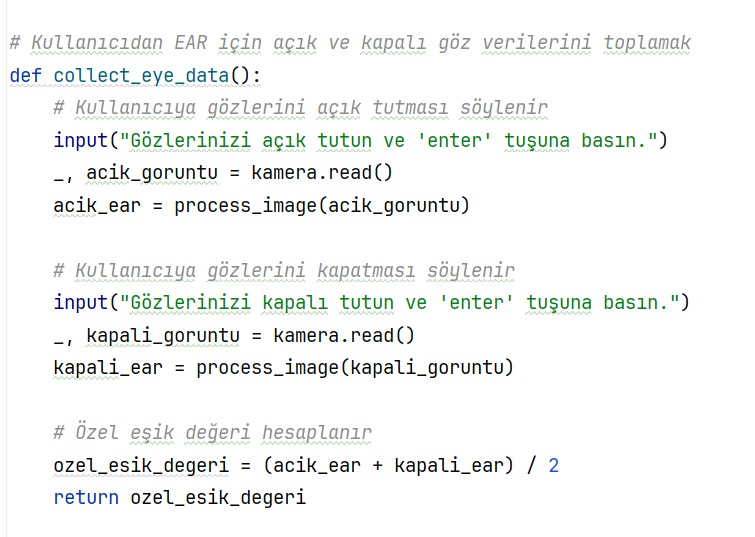
\includegraphics[width=10cm, height=7cm, keepaspectratio]{ozelgoz.jpg}
		\caption{Kişiye özel eşik değerin oluşturulması.}
	\end{figure}
	\begin{figure}
		\centering
		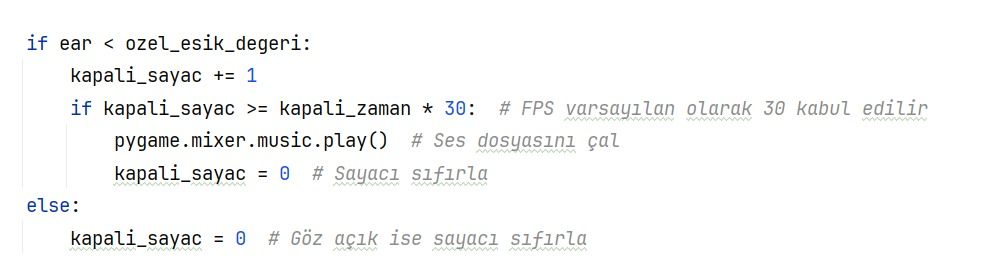
\includegraphics[width=10cm, height=7cm, keepaspectratio]{gozkapaliligi.jpg}
		\caption{Gözlerin kapalı olduğu süreyi hesaplayıp sürücüyü uyarma.}
	\end{figure}\newpage
    \subsection{ Eşik Değere Göre Yorgunluk Durumunun Kategorileştirilmesi} 
	
	\begin{figure}[htbp][!]
		\centering
		\begin{subfigure}{.5\textwidth}
			\centering
			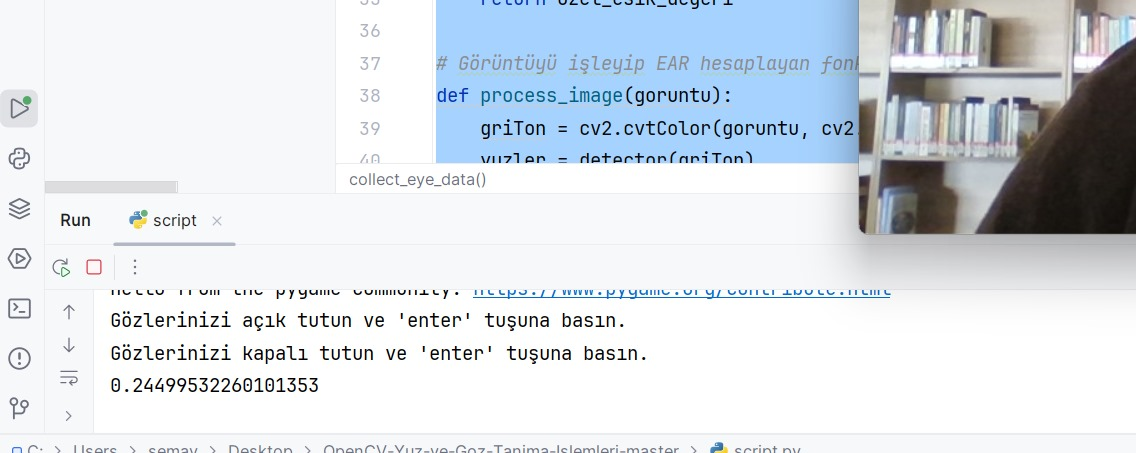
\includegraphics[width=\linewidth,height=4cm]{ goz_esik1.jpg}
			\caption{}
			\label{fig:sub1}
		\end{subfigure}%
		\begin{subfigure}{.5\textwidth}
			\centering
			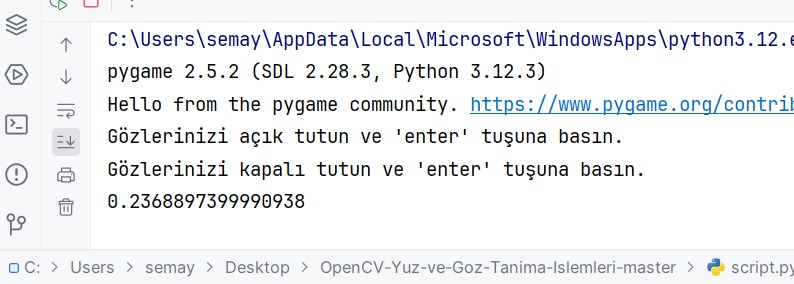
\includegraphics[width=\linewidth,height=4cm]{goz_esik2.jpg}
			\caption{}
			\label{fig:sub2}
		\end{subfigure}
		\caption{Özel eşik değerlerin alınması örnekleri.}
		\label{fig:test}
	\end{figure} \newpage
	\begin{table}[h!]
		\begin{center}
			\caption{Yorgunluk Durumları.}
			\label{tab:table1}
			\begin{tabular}{c|l|l|}
				\textbf{Açıklık Oranı} & \textbf{Tanımlama} & \textbf{Yapılacak}\\
				\hline
				\%60 & Hafif yorgun & 3 tekrarda sürüşe odaklanma uyarısı\\
				\%50 & Tespit edilen eşik değer & Bu değere göre oranlama\\
				\%40 & Çok yorgun & Otele yönlendirme\\
			\end{tabular}
		\end{center}
	\end{table}
	Kişiye özel olarak aldığımız eşik değer aslında tam açık (\%100) açık gözün yarısı değerini almaktaydı. Bu değer kişiye özgü açıklıklar alınıp hesaplandığı için belirli bir değere göre sınıflandırmak yerine bu değerin yüzdeliklerini alarak sınıflandırmak daha sağlıklı sonuçlar doğuracaktır.
	Açıklık oranı \%70 olan bir gözün hafif yorgun olarak belirlenmesi ve bu durumun 3 kez tekrarlanması üzerine "Sürüşe odaklan!" seslendirmesini yapan bir alarmın çalmasına karar verdim. Açıklık oranı \%30 olan bir gözün çok yorgun olarak tanımlanması üzerine aracın hareketine son verilip uygun bir otele yönlendirme yapılmasına karar verdim.\newpage
	\subsection{ Esneme Algılama }
	Göz dışında yorgunluğu tespit etmek için hangi durumların kontrol edileceğine bakıldı. Esneme durumu ve başın pozisyonunu zaten proje kapsamında ama bu hafta nabız alma durumu da araştırıldı. Koltuktan alınabilecek tek nabız diz kapağı arkasından geçen damarda. Bu projenin ilerlenmesi durumunda atılacak adımlardan  biridir bu sebeple ileriy dönük bir araştırma olmuştur. 
	Ayrıca ağız yani esneme durumunu ele alındı. Göz tespit etme ile aynı ilerlendi. Dlib kütüphanesinin sunduğu landmarkları tanımlayarak onları tespit etmek ve bir eşik değere göre esneme var yok hesabı yaptırmak gibi özet geçilebilecek bir aşama gerçekleştirildi.
	\begin{figure}[htbp]
		\centering
		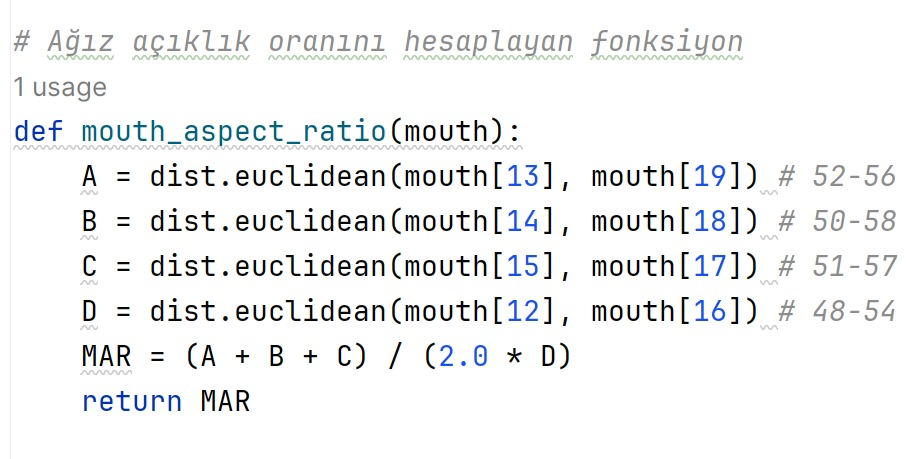
\includegraphics[width=10cm, height=7cm, keepaspectratio]{esneme.jpg}
		\caption{Ağzı tespit etmek için kullanılan fonksiyon.}
	\end{figure}
	\begin{figure}[htbp]
		\centering
		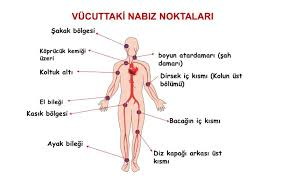
\includegraphics[width=10cm, height=7cm, keepaspectratio]{nabiz.jpeg}
		\caption{Nabız alınabilecek yerler \cite{tuyobank}.}
	\end{figure}\newpage
	\subsection{ Baş Pozisyonu Belirleme }
	Bu hafta başın pozisyonunu da projeye ekleyerek belirlediğim parametreleri tamamlayıp bu parametreler bir arada değerlendirmeye alınmıştır. Başın pozisyonunu belirleyebilmek için öncelikle 2 boyutlu olarak yüzden aldığımız noktaların 3 boyutlu eksene çevrilmesi gerekir. Bu çevirme için bir model kullanıldı. Aynı zamanda bu dönüşümlerin yapılması için de bazı kavramlar bilinmelidir. 
	\begin{figure}[htbp]
		\centering
		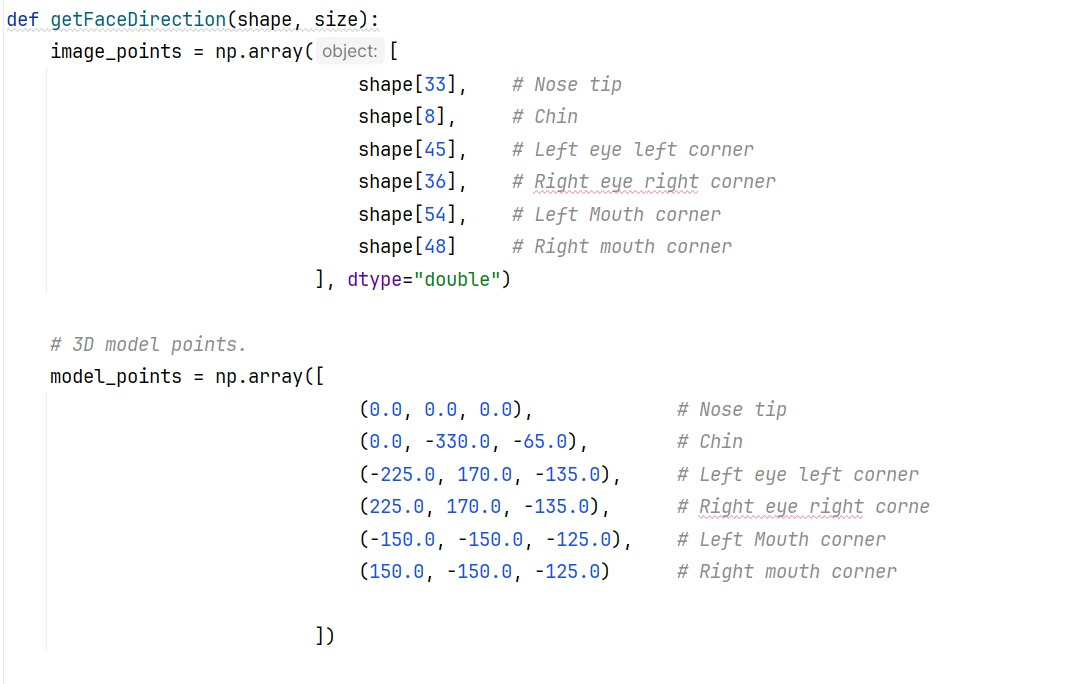
\includegraphics[width=10cm, height=7cm, keepaspectratio]{bastanimlama.jpg}
		\caption{Baş pozisyonunu belirlemek için üç boyutlu model\cite{neelan}.}
	\end{figure}
	\begin{itemize}
		\item Yaw (Y): Yaw, nesnenin yatay eksende (genellikle zemin düzlemi etrafında) dönme hareketini ifade eder. Bir uçağın yatay eksende sola veya sağa dönmesi gibi bir örnektir.
		\item Pitch (P): Pitch, nesnenin dikey eksende (genellikle burnun yukarı veya aşağı doğru hareketi) dönme hareketini ifade eder. Bir uçağın burnunun yukarı veya aşağı doğru eğilmesi gibi bir örnektir.
		\item Roll ®: Roll, nesnenin uzun ekseni etrafında dönme hareketini ifade eder. Bir uçağın kanatlarının bir tarafı yukarı doğru kalkarken diğer tarafı aşağı doğru inmesi gibi bir örnektir.
	\end{itemize}
	Bu kavramlara göre euler açıları hesaplanır. Euler açıları bu proje için başın pozisyonunu belirlemede kullanılmaktadır.
	\begin{figure}[htbp]
		\centering
		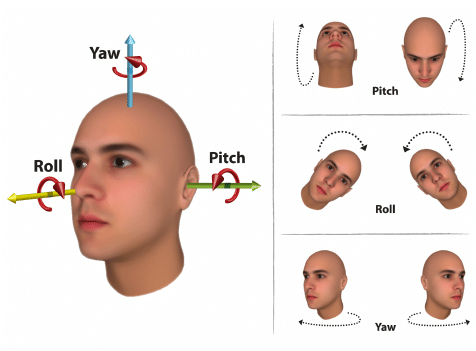
\includegraphics[width=10cm, height=7cm, keepaspectratio]{poz.png}
		\caption{Baş pozisyonunu anlamak için bilinmesi gerekenler.\cite{headpos}.}
	\end{figure}
	
	\begin{figure}[htbp]
		\centering
		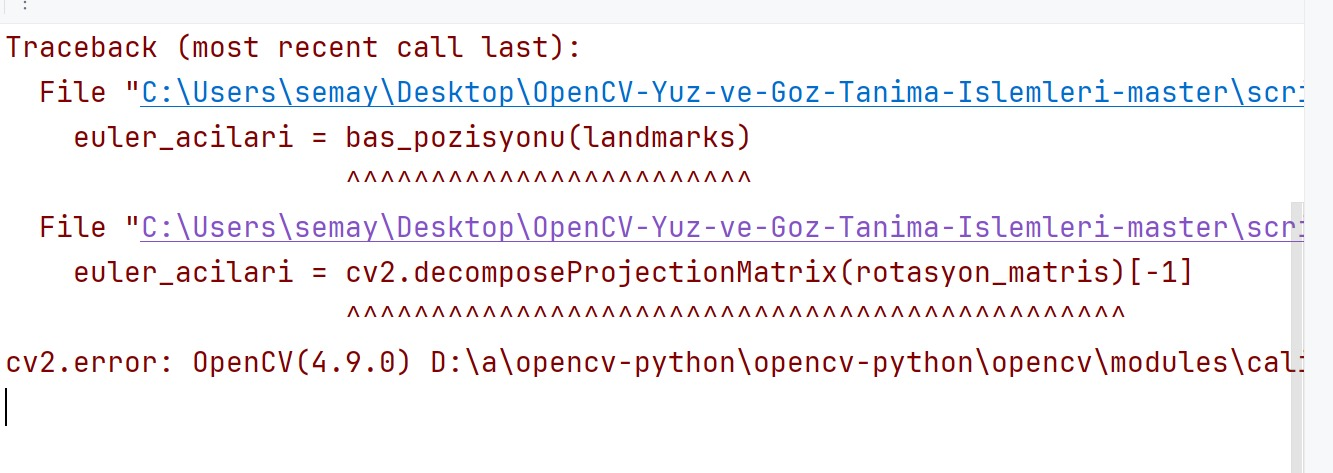
\includegraphics[width=10cm, height=7cm, keepaspectratio]{bashata.jpg}
		\caption{Euler ölçülerinde hata.}
	\end{figure}\newpage
	\subsection{ Baş Pozisyonu Belirleme }
	\begin{itemize}
		\item SolvePnP Fonksiyonu Çağrısı:
		cv2.solvePnP(modelnoktalari, imagepoints, kameramatrisi, bozulmakatsayilari) satırı, 3D model noktalarını (örneğin, bir nesnenin köşe noktaları), görüntüdeki bu noktaların eşlenik 2D görüntü noktalarını, kamera matrisini ve bozulma katsayılarını kullanarak baş pozisyonunu tahmin eder.
		
		\item model noktalari: 3D modelin dünya koordinatlarındaki noktaları.
		\item image points: Görüntüdeki bu noktaların eşlenik 2D görüntü noktaları.
		\item kamera matrisi: Kamera kalibrasyonundan elde edilen iç parametre matrisi.
		\item bozulma katsayilari: Kamera bozulma katsayıları.
		\item Rotasyon Vektörünün Euler Açılarına Dönüştürülmesi:
		cv2.Rodrigues(rotasyonvektor) satırı, rotasyon vektörünü 3x3 rotasyon matrisine dönüştürür.
		Bu matris, nesnenin dünya koordinatlarındaki rotasyonunu temsil eder.
		\item Projeksiyon Matrisinin Oluşturulması:
		projeksiyonmatris = np.hstack((rotasyonmatris, translasyonvektor)) satırı, rotasyonmatrisi ve translasyon vektörünün yatay olarak birleştirilmesiyle projeksiyon matrisini oluşturur.
		\item Projeksiyon matrisi, nesnenin dünya koordinatlarından görüntü koordinatlarına dönüşümü için kullanılır.
		\item Projeksiyon Matrisinin Decompose Edilmesi:
		cv2.decomposeProjectionMatrix(...) satırı, projeksiyon matrisini iç parametre matrisi, rotasyon matrisi, translasyon vektörü, Euler açıları ve diğer bileşenlere ayırır.
		\item euleracilari.ravel() ile Euler açıları döndürülür.\end{itemize}
	\begin{figure}[htbp]
		\centering
		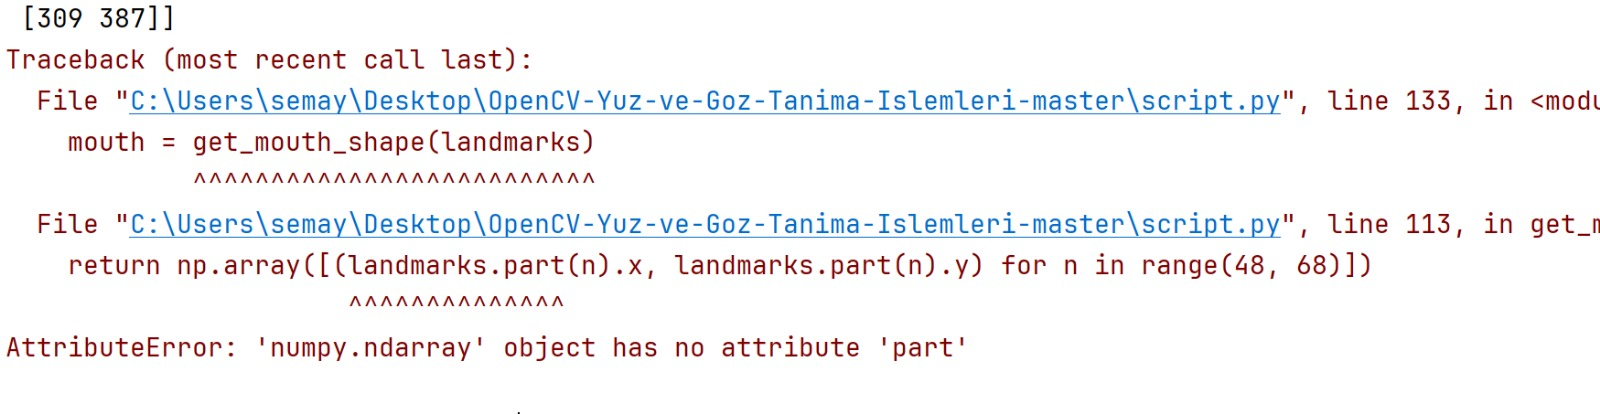
\includegraphics[width=10cm, height=7cm, keepaspectratio]{hataa.jpg}
		\caption{Landmarksların numpya dönüştürme hatası.}
	\end{figure}\begin{figure}[htbp]
		\centering
		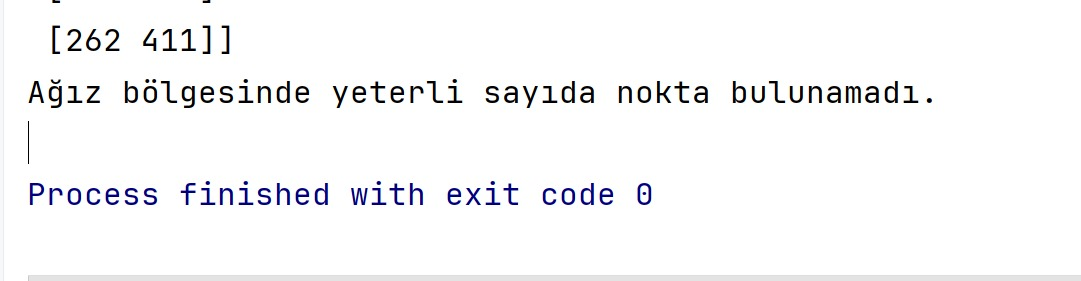
\includegraphics[width=10cm, height=7cm, keepaspectratio]{agizhatasi.jpg}
		\caption{Ağız bölgesi bulunamadı hatası.}
		
	\end{figure}\newpage
		\subsection{ Hataların Giderilip Baş Pozisyonunun Eklenmesi }
		Ağız durumunu hesaplarken alınan hata landmark sayısını kontrol etmek için fonksiyon içerisine yerleştirilen if kontrolü sebebiyle olduğu anlaşılmıştır. Bu kontrolü kaldırınca gerekli esneme algılaması sağlanmaktadır. \par 
		\begin{figure}[!h]
			\centering
			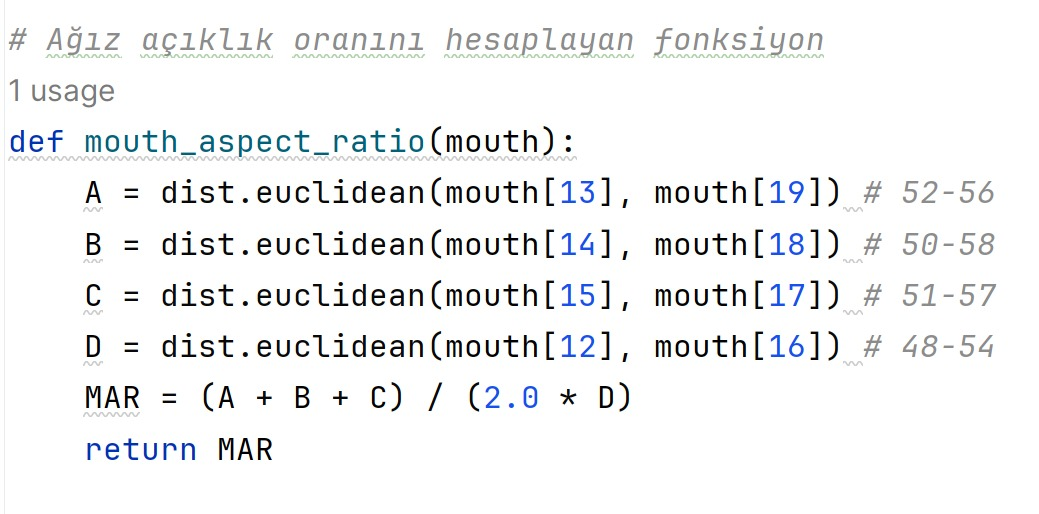
\includegraphics[width=17cm, height=7cm, keepaspectratio]{agizhesap.jpg}
			\caption{Ağız hesabının yapılması.} 
		\end{figure}
		Landmarkların farklı işlemlere tabii tutulması sebebiyle iki farklı landmark tanımlaması uygulandı. Biri baş pozisyonu için rotasyonlar uygulanacak biri de görüntü alınarak ağız ve göz bölgesi için gerekli oranlamalar yapılacak şekilde ayarlanmıştır. \par
		\begin{figure}[!h]
			\centering
			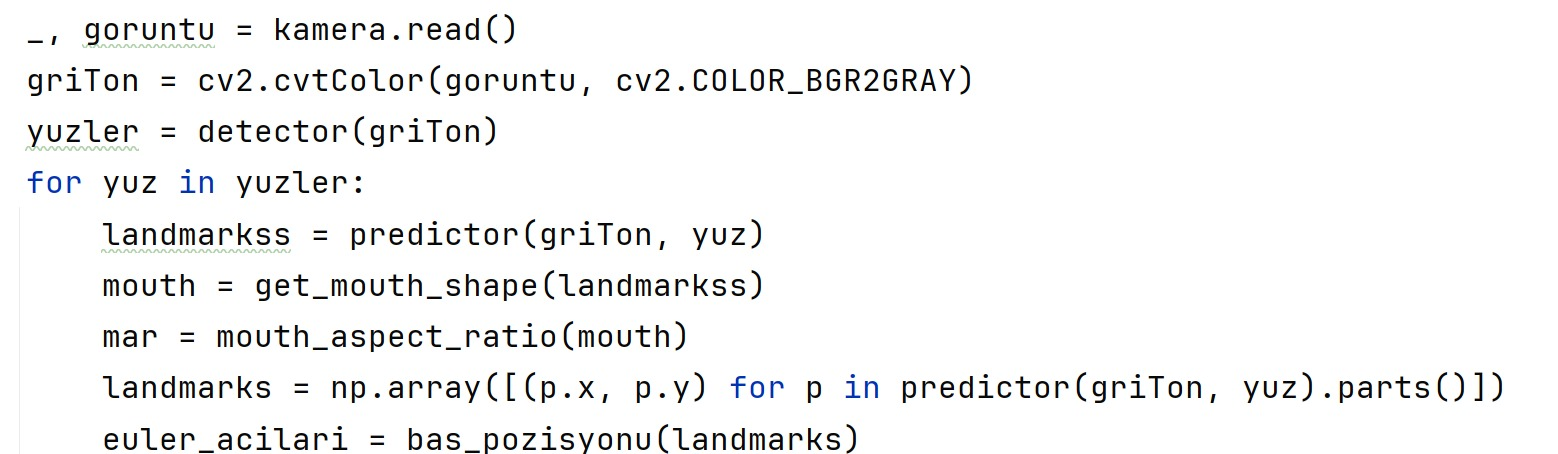
\includegraphics[width=17cm, height=7cm, keepaspectratio]{ikilandmark.jpg}
			\caption{Landmarkların ayarlanması.} 
		\end{figure}
		 Başın poziyonunu algılamak için eklenen fonksiyon ve matris işlemlerinde araştırmalara göre eksik bir bölüm olduğu fark edildi. Rcv2.Rodrigues fonksiyonu ile rotasyon vektöründen rotasyon matrisine dönüşüm yapılması gerekmektedir.\newpage
		\begin{figure}[!h]
			\centering
			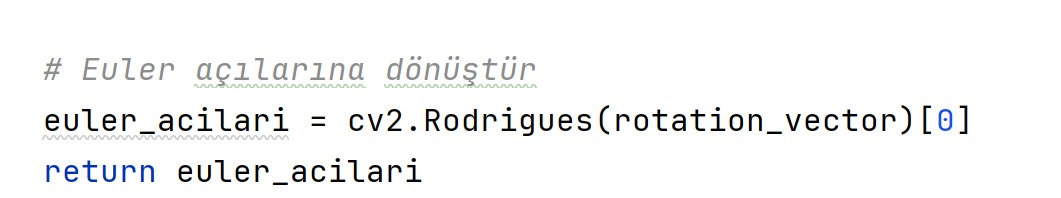
\includegraphics[width=17cm, height=7cm, keepaspectratio]{redkullan.jpg}
			\caption{Göz tespiti için Dlib kütüphanesinin kullandığı landmark değerleri.} 
		\end{figure}
		Gerekli dönüşümler yapıldıktan sonra uyuklama kontrolü için başın pozisyonlarından pitch değeri kullanılmaktadır.Bu değer dışındaki değer ileriye dönük olarak kullanılabileceği gibi şu an pitch değeri proje için yeterli bir kontrol sağlamaktadır.\par 
		 \begin{figure}[!h]
			\centering
			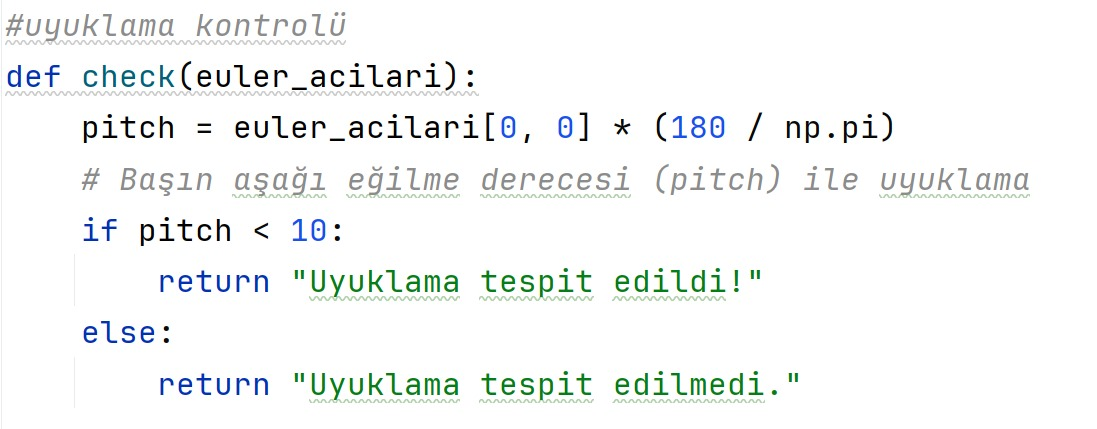
\includegraphics[width=17cm, height=7cm, keepaspectratio]{uyuklamakont.jpg}
			\caption{Göz tespiti için Dlib kütüphanesinin kullandığı landmark değerleri.} 
		\end{figure}
		 
		 
	\section{Sonuç}

	Projede sürücülerin yorgunluk durumlarının algılanması sorununa çözüm üretilmiştir. Göz kapalılık durumu tespiti, ağza bakılarak uykululuk tespiti ve başın pozisyonuyla vücut duruşu tespiti sağlandı. Göz tespitinin kişiye özel olması sebebiyle yüksek bir başarım oranı sağlanmıştır. Diğer çalışmalarda geleneksel yöntemle ilerlenmeyip landmark konusu kullanılmamıştır. Bu nedenle Haarcascade yöntemi ile referans alınan projeler olsa da ilerlemelerin sağlanmadığı görülmüştür. Başın pozisyonu, esneme algılama ve kişiye özel göz tespiti uygulamaları farklılık göstermektedir.
\bibliographystyle{ieeetr}
\bibliography{ref.bib} %\cite{aayushrai,bulentsezen,neelanjan00,researchgate,mrl,ieeedata,dasar_haartrain,amos2018,onursahin,eadali,superthinking,cnnnedir,cnnnedirtek,copilot,neelan,researchgate,tuyobank}
\newpage 	
	
\end{document}          
